\documentclass[a4paper]{article}
\usepackage[left=2.1cm, right=2.1cm, top=2.1cm]{geometry}
\usepackage{lipsum}
\usepackage{tikzpagenodes}
\usepackage{pgfplots}
\usepackage{tikz}
\usepackage{tikz-3dplot}
\usetikzlibrary{arrows,decorations.pathmorphing,backgrounds,positioning,fit,matrix}
\pgfplotsset{compat=1.8}
\usepackage{graphics} % for pdf, bitmapped graphics files
\usepackage{epsfig} % for postscript graphics files
\usepackage[colorlinks=true,citecolor=green]{hyperref}
\usepackage{cite}
\usepackage{amsmath,amssymb,amsfonts}
\usepackage{algorithmic}
\usepackage{graphicx}
\usepackage{url}
\usepackage{cite}
\usepackage{bm}
\usepackage{pbox}
\usepackage{siunitx,booktabs,etoolbox}
\usepackage{ulem}
\usepackage[framed,numbered,autolinebreaks,useliterate]{mcode}
\usepackage{filecontents}
%\usepackage{bigfoot} % to allow verbatim in footnote


\def\BibTeX{{\rm B\kern-.05em{\sc i\kern-.025em b}\kern-.08em
    T\kern-.1667em\lower.7ex\hbox{E}\kern-.125emX}}

\begin{filecontents*}{ipm1.m}
imread;
rgb2gray;
im2double;
filter2;
imfilter;
conv2;
imshow;
\end{filecontents*}


\begin{document}

\title{Exercise on Harris Feature Detector}
\author{xiahaa@space.dtu.dk}
\maketitle%%

In this exercise, you will work on Harris corner detector.

\section{Harris corner}
\begin{enumerate}
\item compute horizontal and vertical first order derivative: you can use any template like Prewitt, Sobel, or DoG. 
\item Compute three intermediate images $I_x^2$, $I_{xy}$, $I_y^2$, show them.
\item Smooth them ($I_x^2$, $I_{xy}$, $I_y^2$) with the Gaussian template.
\item for every pixel, find $\mathbf{C}=\left[\begin{matrix}
Ix^2 & I_{xy} \\ I_{xy} & I_{y}^2
\end{matrix}\right]$.
\item compute $det(\mathbf{C})-\mathit{k}trace(\mathbf{C})^2$.
\item threshold to find corners.
\item apply Non-maxima suppression.
\end{enumerate}

\begin{figure*}[!b]
\centering
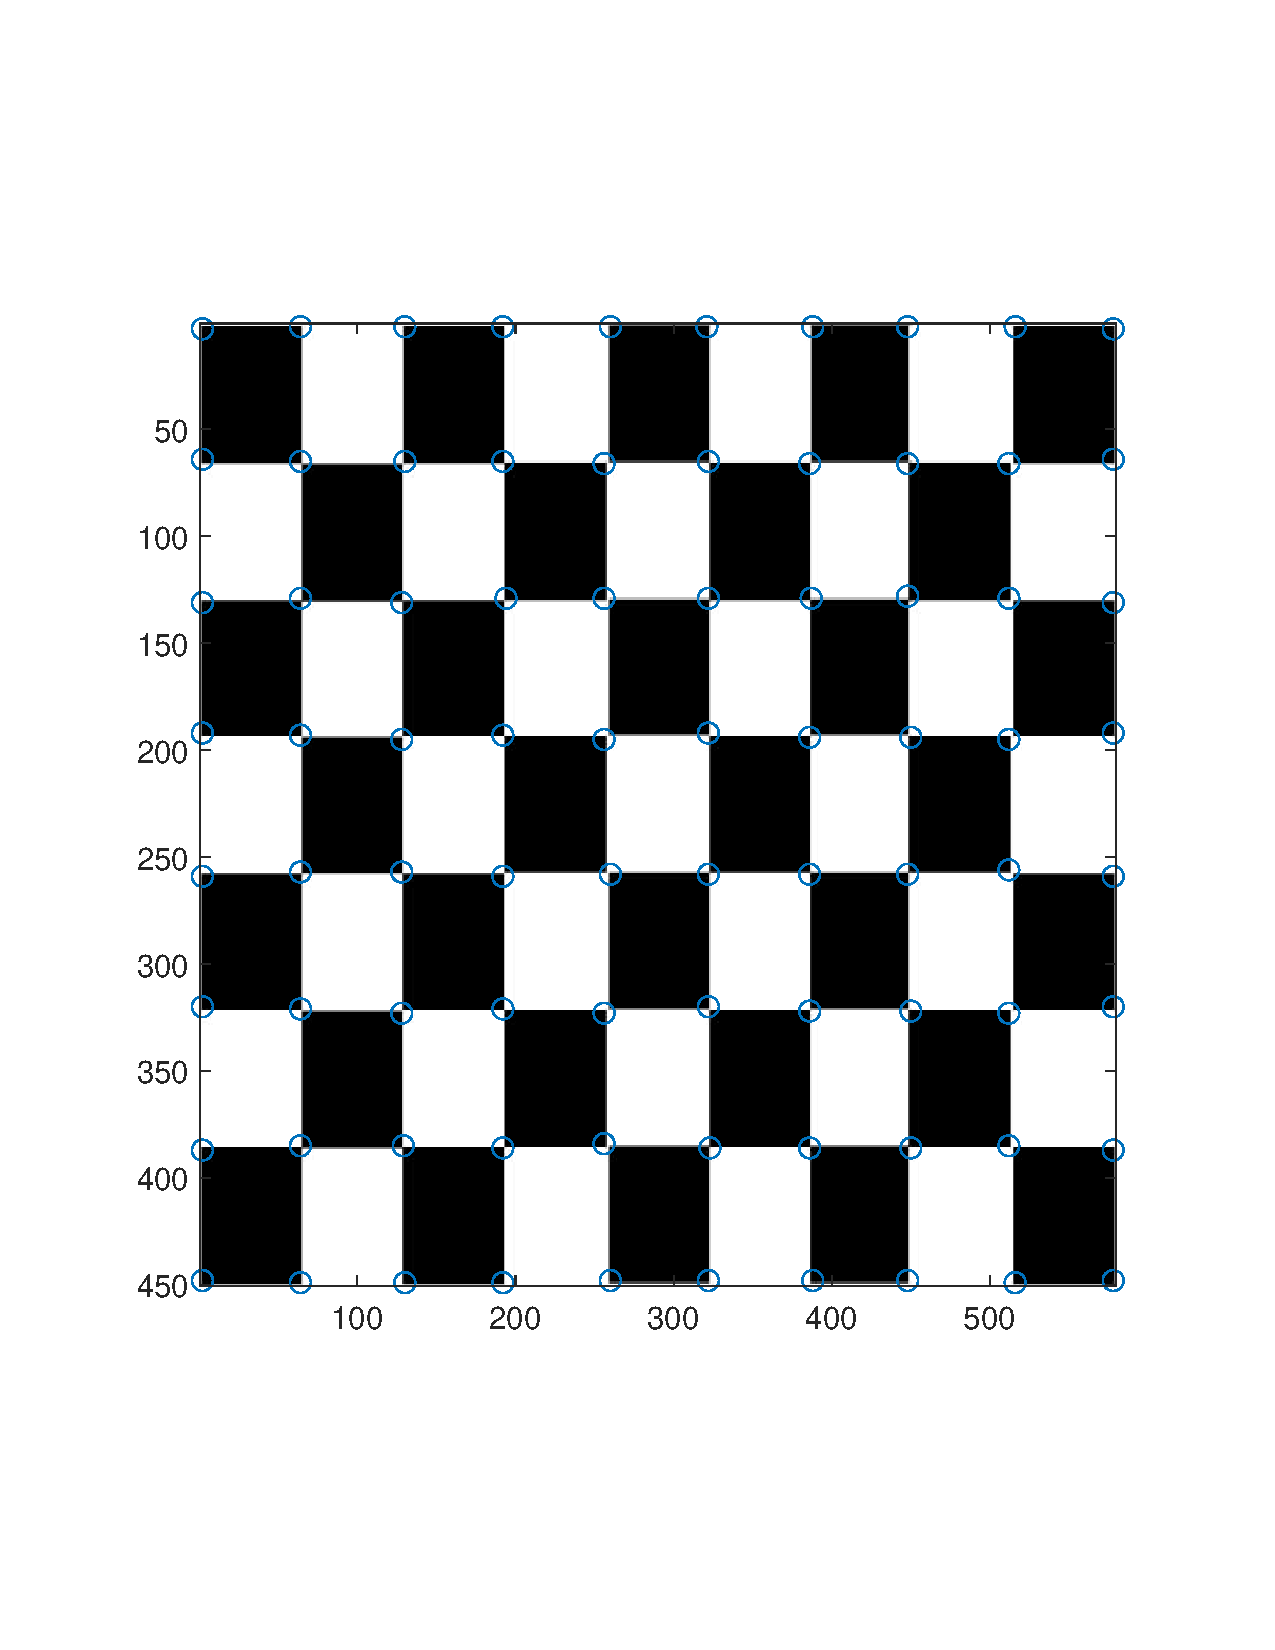
\includegraphics[scale=0.3]{figures/harris}
\caption{Example of result.}
\end{figure*}

\section{Useful functions}
\lstinputlisting{ipm1.m}




 
\bibliography{hand_eye_calibration} 
\bibliographystyle{ieeetr}

\end{document}